\chapter{Исследовательская часть}

\section{Технические характеристики}

Технические характеристики устройства, на котором выполнялись замеры по времени:

\begin{itemize}
    \item Процессор: Intel i5-1035G1 (8) @ 3.600GHz.
    \item Оперативная память: 16 ГБайт.
    \item Операционная система: Manjaro Linux x86\_64 (версия ядра Linux 5.15.131-1-MANJARO).
\end{itemize}

Во время проведения измерений времени ноутбук был подключен к сети электропитания и был нагружен только системными приложениями.

\section{Демонстрация работы программы}

На рисунке \ref{fig:prog-demo} показан пример работы разработанной программы для случая, когда пользователь выбирает действие <<Запуск алгоритмов поиска расстояния Левенштейна>> и вводит строки <<кот>> и <<кошка>>.

\clearpage
\begin{figure}[h]
    \centering
    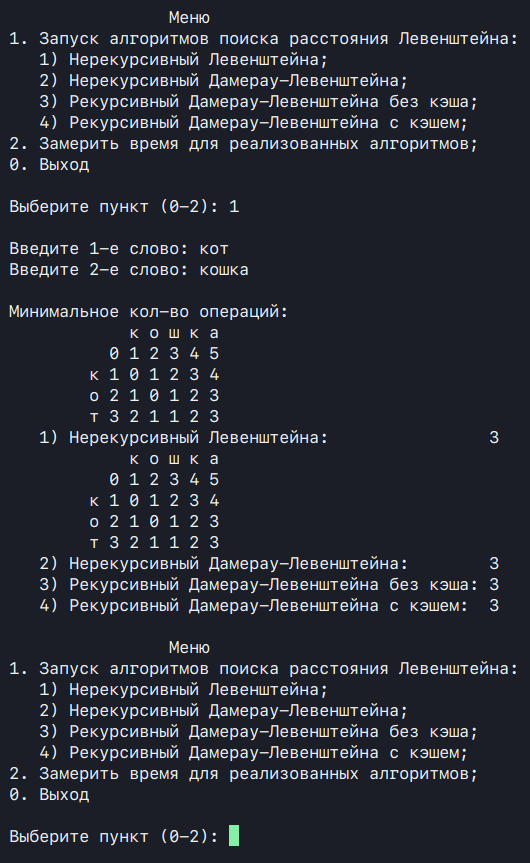
\includegraphics[height=0.6\textheight]{images/prog_demo.png}
    \caption{Демонстрация работы программы}
    \label{fig:prog-demo}
\end{figure}

\section{Временные характеристики}

Исследование временных характеристик алгоритмов производилось на случайно сгенерированных строках длинами от 1 до 10, длины изме\-няются с шагом 1. Для нерекурсивных алгоритмов отдельно производилось сравнение на строках длинами от 20 до 100 с шагом изменения длины 10. Во избежание погрешности измерения для каждой строки производились 50 раз, затем вычислялось среднее арифметическое всех полученных значений времени.

\begin{figure}[H]
    \centering
    \includesvg[width=1.0\textwidth]{images/nonrec.svg}
    \caption{Результат измерений времени работы нерекурсивных реализаций алгоритмов поиска расстояний Левенштейна и Дамерау\,--\,Левенштейна}
    \label{fig:nonrec-time}
\end{figure}

\begin{figure}[H]
    \centering
    \includesvg[width=1.0\textwidth]{images/rec.svg}
    \caption{Результат измерений времени работы рекурсивный реализаций алгоритма поиска расстояния Дамерау\,--\,Левенштейна}
    \label{fig:rec-time}
\end{figure}

\section{Характеристики по памяти}

Введем следующие обозначения:

\begin{itemize}
    \item $m$~--- длина строки $S_1$;
    \item $n$~--- длина строки $S_2$;
    \item $size(v)$~--- функция, вычисляющая размер входного параметра $v$ в байтах;
    \item $char$~--- тип данных, используемый для хранения символа строки;
    \item $int$~--- целочисленный тип данных.
\end{itemize}

Теоретически оценим объем используемой памяти итеративной реа\-лизацией алгоритма поиска расстояния Левенштейна:

\begin{multline}
    M_{LevIter} = (m + 1) \cdot (n + 1) \cdot size(int) + (m + n) \cdot size(char) + \\
    + size(int**) + (m + 1) \cdot size(int*) + \\
    + 3 \cdot size(int) + 2 \cdot size(int),
\end{multline}

\noindent где:
\begin{itemize}
    \item $(m + 1) \cdot (n + 1) \cdot size(int)$~--- размер матрицы;
    \item $size(int**)$~--- размер указателя на матрицу;
    \item $(m + 1) \cdot size(int*)$~--- размер указателей на строки матрицы;
    \item $(m + n) \cdot size(char)$~--- размер двух входных строк;
    \item $2 \cdot size(int)$~--- размер переменных, хранящих длину строк;
    \item $3 \cdot size(int)$~--- размер переменных цикла $i$, $j$ и промежуточной переменной $cost$.
\end{itemize}

Для алгоритма поиска расстояния Дамерау\,--\,Левенштейна теорети\-ческая оценка объема используемой памяти идентична.

Произведем оценку затрат по памяти для рекурсивных реализаций алгоритма нахождения расстояния Дамерау\,--\,Левенштейна.

Для 

\section{Вывод}
